\chapter{Contesto aziendale}
\label{cap:contestoAziendale}

\section{Wintech S.p.A.}
\noindent Winning Technologies, in sigla Wintech S.p.A., venne fondata nel 1987 dall'attuale amministratore delegato Massimo Gallotta.\\
Essa si occupa di \gls{system integration} nell'ambito delle \glslink{ICT}{tecnologie dell'informazione e della comunicazione}, ovvero unisce ed integra diverse tecnologie e sistemi informatici al fine di ottenere un prodotto coordinato e maggiormente gestibile.\\\\
L'azienda, la quale conta più di 90 dipendenti, ha sede principale situata a Padova ma, grazie al suo sviluppo, ha acquisito filiali a Milano e a Bassano del Grappa.\\
Wintech ha stretto svariate \emph{partnership} con aziende \emph{leader} di mercato come IBM, Microsoft e HP grazie anche alla propria affidabilità e solidità finanziaria.\\ 
Inoltre, possiede diverse società partecipate, tra cui \glslink{Sistemi}{Sistemi S.p.A.}, con le quali è attiva una forte collaborazione.\\
\begin{figure}[htbp] 
    \centering 
    
\includegraphics[width=0.5\columnwidth]{espansioneTerritoriale} 
    \caption{Espansione territoriale di Wintech comprese le sedi partecipate.}
    \label{fig:espansioneTerritoriale}
    \vspace{1mm}
    Fonte: \url{https://www.wintech.it/chi-siamo/}.
\end{figure}
\noindent I clienti di Wintech comprendono grandi imprese (tra cui BMW, Helvetia e Lindt), \glslink{PMI}{Piccole e Medie Imprese}, professionisti, aziende assicurative e imprese finanziarie.\\

\section{Servizi e prodotti}
\subsection{Servizi}
I servizi offerti da Wintech comprendono diverse aree tecnologiche:
\begin{itemize}
	\item \textbf{Infrastrutture \gls{IT}}: vengono offerte soluzioni per modernizzare e gestire le infrastrutture aziendali sfruttando tecnologie basate sulla rete internet (\gls{cloud}), progettazioni di connessioni di rete, sia di area contenuta (\gls{LAN}), che con maggiore portata (\gls{WAN}), gestione di \emph{backup} sicuri e supporto \gls{IT}, ovvero relativo all'ambito delle tecnologie dell'informazione, conforme agli standard definiti nelle linee guida raccolte nell'\glslink{ITIL}{Information Technology Infrastructure Library}. 
	\item \textbf{Automazione di processi di \emph{Business}}: vengono forniti strumenti per automatizzare i processi aziendali come flussi approvativi, gestione documentale e metodologie \gls{DevOps}. Queste ultime enfatizzano l'automazione al fine di ridurre i tempi e i costi di sviluppo aumentando la qualità dei prodotti realizzati.  
	\begin{figure}[htbp] 
        \centering 
        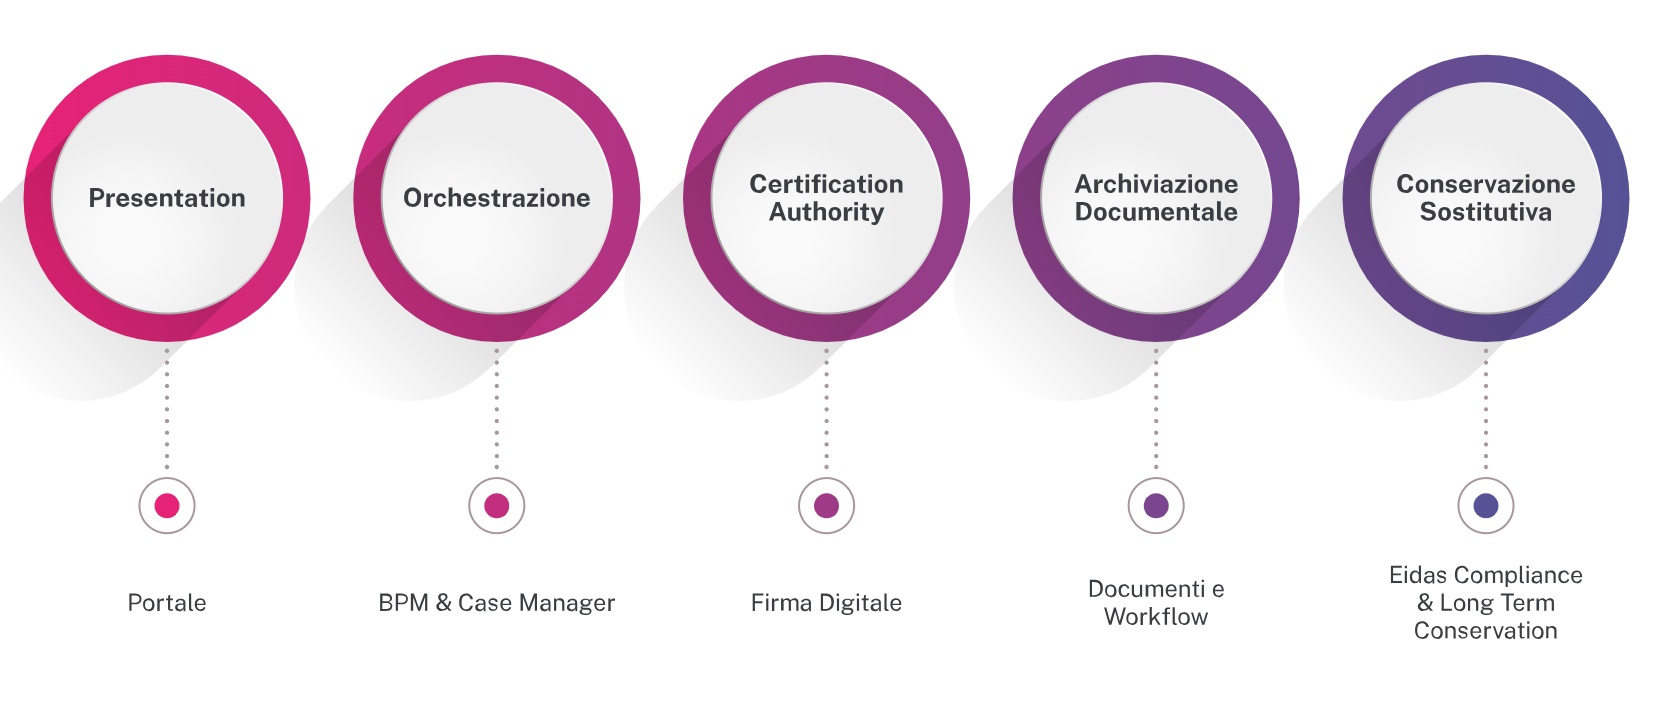
\includegraphics[width=1\columnwidth]{digitalTrasformation}
        \caption{Soluzioni per l'automazione di processi.} 
        \label{fig:digitalTransformation}
        Fonte: \url{https://www.wintech.it/business-automation/}.
    \end{figure}
    \item \textbf{\emph{Cyber} sicurezza}: per garantire la continuità aziendale viene fornita protezione contro i rischi informatici mediante difesa delle reti e dei dispositivi, segmentazione della rete, servizi gestiti e soluzioni di \gls{disaster recovery}. Queste ultime si riferiscono a processi di ripristino dei dati persi a seguito di un evento dannoso.
	\item \textbf{Soluzioni \gls{ERP}}: vengono sviluppati sistemi per la gestione delle risorse aziendali come automazioni per le Risorse Umane, sistema di gestione dei clienti (\emph{Customer Relationship Management}), soluzioni gestionali per la produzione industriale, soluzioni per industria 4.0/5.0.\\\\
\end{itemize}
Viene offerta consulenza al cliente al fine di fornire supporto tecnico e comprendere le sue necessità.\\
Successivamente viene identificata una soluzione adeguata, la quale può essere sviluppata partendo da un prodotto aziendale già consolidato apportando le opportune personalizzazioni, oppure realizzando un prodotto nuovo.\\
In seguito allo sviluppo di un prodotto, vengono forniti servizi di formazione, assistenza e manutenzione dello stesso.\\

\subsection{Prodotti}
I principali prodotti offerti dall'azienda sono: 

\subsubsection*{Spring}
Supporta le \gls{PMI} gestendo le informazioni relative alle attività di diverse aree aziendali come: 

\begin{itemize}
    \item Amministrativa 
    \item Vendite 
    \item Acquisti 
    \item Logistica e magazzino
    \item Analisi e \emph{reporting}
    \item Gestione documentale
\end{itemize}

\subsubsection*{Studio}
Offre servizi legati all'organizzazione e alla gestione dello studio professionale come:
\begin{itemize}
    \item Calendari condivisi  
    \item Gestione efficiente delle pratiche 
    \item Emissione di parcelle  
    \item Fatture elettroniche 
\end{itemize}

\subsubsection*{Job}
Fornisce servizi legati alla gestione del personale come: 
\begin{itemize}
    \item Gestione delle presenze  
    \item Amministrazione delle Risorse Umane  
    \item Elaborazioni dei cedolini 
    \item Analisi sui costi del personale
\end{itemize}

\subsubsection*{Sportello}
Propone servizi legati alla gestione dei clienti come:  
\begin{itemize}
    \item Gestione della fatturazione online 
    \item Gestione degli incassi e dei pagamenti 
    \item Condivisione, validazione e conservazione digitale dei documenti  
\end{itemize}

\subsubsection*{eSolver}
Mette a disposizione servizi legati alla gestione dei processi per aziende di produzione, di servizi, di commercio all'ingrosso e al dettaglio. 
Le principali funzionalità comprendono: 
\begin{itemize}
    \item Amministrazione e finanza 
    \item Acquisti e rapporti di fornitura 
    \item Vendite e attività commerciale 
    \item Logistica
    \item Archiviazione e conservazione documentale
    \item Gestione risorse produttive 
    \item Produzione manifatturiera  
    \item Controllo di gestione 
    \item \emph{Reporting} e analisi 
\end{itemize}

\subsubsection*{Profis}
Fornisce servizi legati alle aree di attività dello studio del commercialista come: 
\begin{itemize}
    \item Area fiscale dei bilanci 
    \item Contabilità e digitalizzazione dei processi di fatturazione  
\end{itemize}
\begin{figure}[htbp] 
    \centering 
    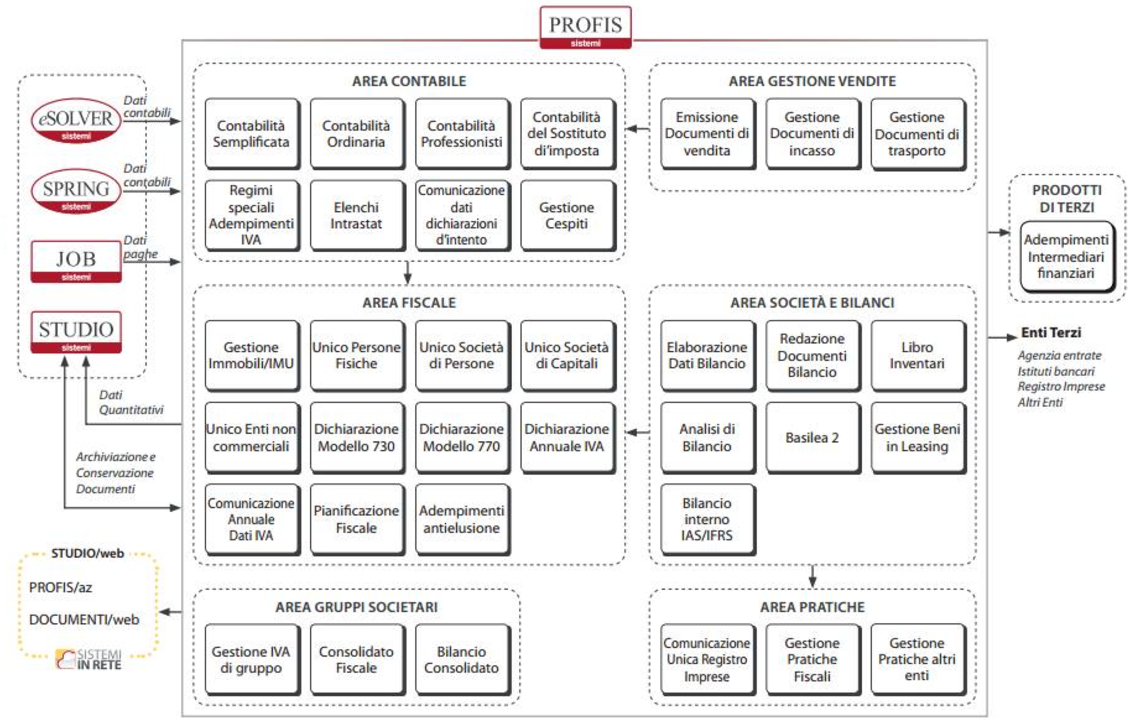
\includegraphics[width=1\columnwidth]{strutturaProfis}
    \caption{Struttura dei moduli di Profis.}
    \label{fig:strutturaProfis}
\end{figure}


\subsubsection*{WOW}
\label{WOW}
“\emph{World Of Wintech}” (WOW) viene considerato non solo un utile prodotto per i clienti, ma soprattutto un potente strumento gestionale aziendale utilizzato da tutti i dipendenti.\\ 
Essa è una soluzione basata interamente sul \gls{cloud}, altamente personalizzabile ed integrabile con i sistemi gestionali e applicativi già in possesso da un cliente.\\
WOW permette di utilizzare svariati moduli gestionali in un'unica interfaccia utente e di gestire i documenti grazie alla piattaforma FileNet - IBM, permettendo operazioni di collaborazione in tempo reale.\\
Quest'ultima è una piattaforma di \gls{back-end}, ovvero parte del \emph{software} generalmente non visibile all'utente, responsabile della sicurezza e gestione dei dati e della relativa logica.\\\\
I principali moduli che lo compongono sono: 

\begin{itemize}
    \item \textbf{Home}: organizzazione delle risorse aziendali interne. 
    \item \textbf{Opportunità}: tracciamento delle trattative commerciali. 
    \item \textbf{Marketing}: gestione delle azioni di \emph{marketing}. 
    \item \textbf{Campagne commerciali}: assegnazione delle attività e gestione campagne commerciali.
    \item \textbf{Anagrafiche}: profilazione clienti e contatti aziendali. 
    \item \textbf{Commesse}: gestione informazioni anagrafiche di commessa al fine di categorizzare i documenti archiviati.
    \item \textbf{Add-In O365}: connessione con Outlook365 per l'archiviazione dei messaggi di posta elettronica.
    \item \textbf{Registro accessi}: gestione degli accessi in azienda da parte di ospiti e collaboratori.
    \item \textbf{Documenti}: archiviazione dei documenti mediante la piattaforma IBM e l'integrazione con Microsoft365.\\
\end{itemize}
\hyperref[WOW]{WOW} si integra con il prodotto eSolver al fine di gestire tutte le principali aree di interesse aziendale.\\

\section{Processi aziendali}
\subsection{Metodologia \emph{Agile}}
Grazie all'utilizzo di \hyperref[WOW]{WOW} e alle politiche aziendali, è molto forte la collaborazione e la condivisione di informazioni tra i dipendenti. Il tutto è reso maggiormente dinamico ed efficiente grazie all'adozione della metodologia \emph{Agile}.\\
Essa è un approccio alla gestione progettuale che promuove la collaborazione e il dialogo tra membri del \emph{team} e con i clienti al fine di condividere costantemente \emph{feedback} e rispondere prontamente ai cambiamenti.\\\\
I quattro valori che descrivono la filosofia \emph{Agile} sono:
\begin{itemize}
    \item Gli individui e le interazioni più che i processi e gli strumenti 
    \item Il \emph{software} funzionante più che la documentazione esaustiva  
    \item La collaborazione col cliente più che la negoziazione del contratto 
    \item Rispondere al cambiamento più che seguire un piano\\\\
\end{itemize}
In Wintech viene adottato il \emph{framework} \emph{Agile} “\emph{Scrum}” per la gestione dei progetti.\\
Esso prevede una divisione temporale dell'avanzamento dei lavori organizzata per “\emph{Sprint}”, i quali in azienda hanno una durata variabile di circa un mese ciascuno.\\
All'inizio di ogni \emph{Sprint} esso viene pianificato definendo tutte le attività da svolgere.\\\\
Quotidianamente è previsto un breve incontro tra i membri del \emph{team} in modo da confrontarsi sullo stato di avanzamento dei lavori e su eventuali problemi riscontrati.\\
Al termine dello \emph{Sprint} viene fatta una revisione per analizzare i risultati ottenuti e avviene un'analisi retrospettiva al fine di far emergere gli aspetti positivi e quelli migliorabili riguardo il suo svolgimento, la collaborazione del \emph{team} e l'utilizzo degli strumenti forniti.\\\\


\noindent Il \emph{framework} adottato prevede tre figure fondamentali: 
\subsubsection*{Product Owner}
Colui che si focalizza sulle esigenze aziendali, dei clienti e di mercato. Egli definisce le attività da compiere e la loro priorità.
In azienda tale ruolo è responsabilità del \gls{project manager}, ovvero colui che viene identificato come il responsabile di progetto di riferimento. 

\subsubsection*{Scrum Master}
Colui che organizza le risorse per la pianificazione dello \emph{Sprint} e coordina lo svolgimento delle procedure e cerimonie \emph{Scrum} garantendo una corretta applicazione delle sue filosofie.
In azienda tale ruolo è responsabilità del \gls{project manager}. 

\subsubsection*{Team di sviluppo}
Il gruppo di lavoro, il quale gode di una buona autonomia nell'avanzamento e assegnazione dei lavori, è composto da una decina di membri con diverse competenze. Tra loro è presente una forte collaborazione e dialogo in modo da condividere le proprie conoscenze e progredire con lo stato dei lavori in modo efficace.\\\\\\\\
\begin{figure}[htbp] 
    \centering 
    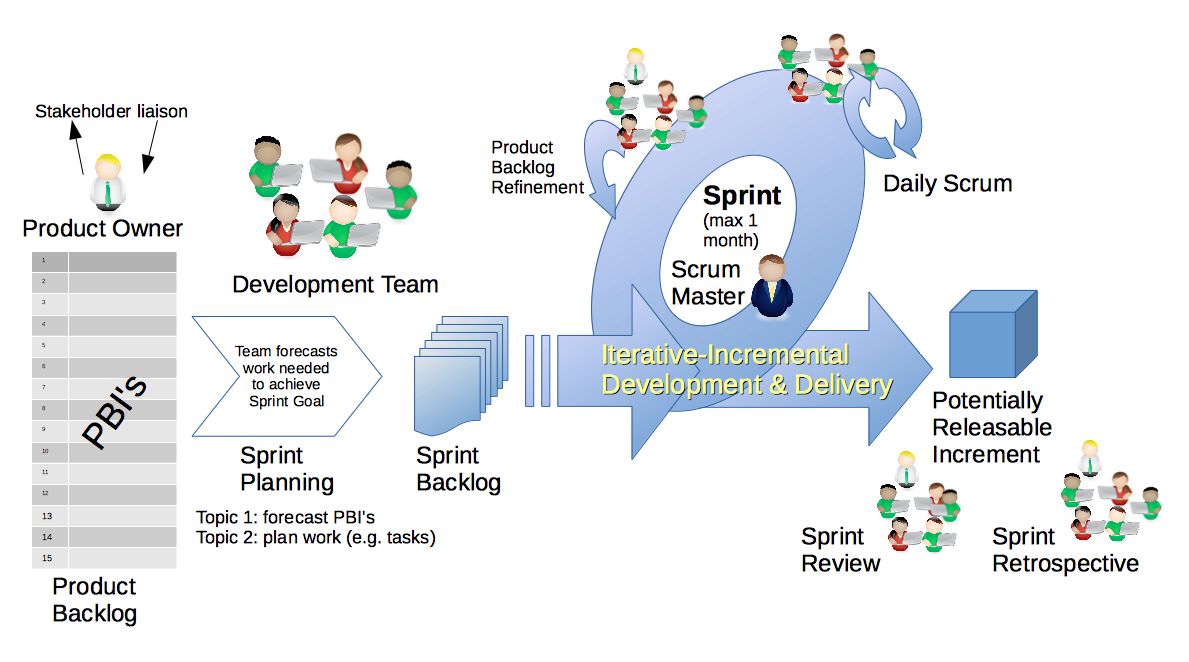
\includegraphics[width=1\columnwidth]{scrum_Framework} 
    \caption{Organizzazione framework Scrum.}
    \label{fig:scrum_framework}
    \vspace{1mm}
    Fonte: \url{https://commons.wikimedia.org/wiki/File:Scrum_Framework.png}.
\end{figure}
\newpage \noindent In Wintech i ruoli \emph{Scrum} non sono rappresentati sempre dalle stesse figure bensì vengono ricoperti da individui differenti seguendo un preciso ordine e una rotazione specifica.\\
Inoltre, le cerimonie possono avvenire per sottogruppi in base alle circostanze e alle esigenze incontrate. Per esempio, può capitare che avvengano determinate cerimonie tra \emph{project manager} e gli elementi del \emph{team} più esperti mentre, in un secondo momento, avvenga un ulteriore incontro tra tali \emph{senior} e il resto del \emph{team}.\\
Durante questi incontri, a sviluppatori con poca esperienza o risorse esterne non viene necessariamente richiesto di contribuire fornendo la propria visione relativamente alla decisione dei \emph{task} o alla personale analisi su dati e stime mostrate.\\\\

\subsection{Unità operative}

\noindent Le principali divisioni lavorative in cui è strutturata Wintech sono:

\subsubsection*{Applicazioni}
Formata da un gruppo di consulenti applicativi i quali si occupano di consulenza, integrazione e assistenza sui \emph{software} gestionali aziendali nei confronti dei clienti. 

\subsubsection*{Soluzioni}
Comprende programmatori con competenze trasversali in grado di definire, progettare e realizzare le soluzioni necessarie per soddisfare le richieste dei clienti. 

\subsubsection*{Tecnologie}
Al suo interno persone con competenza sistemistica monitorano e gestiscono i \emph{server} aziendali al fine di garantire continuità operativa a tutti i clienti in \gls{cloud}. Il personale si dedica all'assistenza dei clienti sia da remoto che in sede, proponendo componenti \emph{hardware} adatte alle esigenze. 

\subsubsection*{Ricerca e Sviluppo}
Composta da un \emph{team} di programmatori avente una maggiore libertà in termini di sperimentazione tecnologica e metodologica. Durante il corso dello \emph{stage} ho fatto parte di questa \gls{unità operativa}.\\
\begin{figure}[htbp] 
    \centering 
    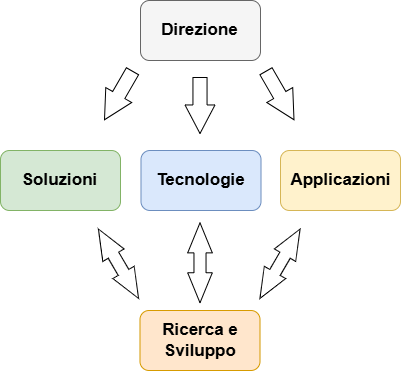
\includegraphics[width=0.6\columnwidth]{rapportoBU}
    \caption{Rapporto tra le unità operative.} 
    \label{fig:rapportoBU}
\end{figure}
\subsection{Documenti e Certificazioni}
Durante il ciclo di vita di un progetto vengono generati un insieme di documenti atti a descriverlo e a normare le attività in esso svolte.\\
I documenti che descrivono le procedure e i metodi da adottare per garantire sicurezza e qualità al prodotto sono spesso comuni a più progetti, pertanto, essi vengono duplicati e modificati solo nei casi in cui le tecnologie o le circostanze rendono tali modifiche necessarie.\\
Tra questi documenti ci sono i “Documenti di sviluppo sicuro” i quali normano le procedure legate al ciclo di vita del progetto e alle buone pratiche da adottare.\\ 
Differentemente, alcuni documenti devono venire prodotti più specificatamente per ogni progetto. Tra questi sono presenti: l'analisi dei requisiti, lo schema architetturale, le criticità, il manuale utente e di installazione, il verbale di collaudo e il “\emph{Bill of Material}” contenente tutti i \emph{software} di terze parti necessari all'utilizzo.\\\\
I processi aziendali definiti hanno reso possibile l'ottenimento delle certificazioni UNI CEI ISO/IEC 27001:2017 IAF 33 e UNI EN ISO 9001:2015 IAF 33,39,37 le quali attestano rispettivamente la conformità del sistema di gestione per la sicurezza delle informazioni e la qualità della gestione aziendale in termini di efficacia, efficienza e soddisfazione dei clienti.\\\\


\section{Tecnologie utilizzate}
All'interno dell'azienda, più specificatamente nelle \glslink{unità operativa}{unità operative} Ricerca e Sviluppo e Soluzioni, vengono utilizzate le seguenti tecnologie: 
\begin{itemize}
    \item Per la pianificazione e il monitoraggio delle attività progettuali vengono utilizzate piattaforme dedicate come Microsoft Planner e Taiga, strumenti versatili che permettono di organizzare le attività ad alto livello (\glslink{caso d'uso}{casi d'uso}) e i \emph{task} in modo collaborativo ed efficiente. 
    \begin{figure}[htbp] 
        \centering 
        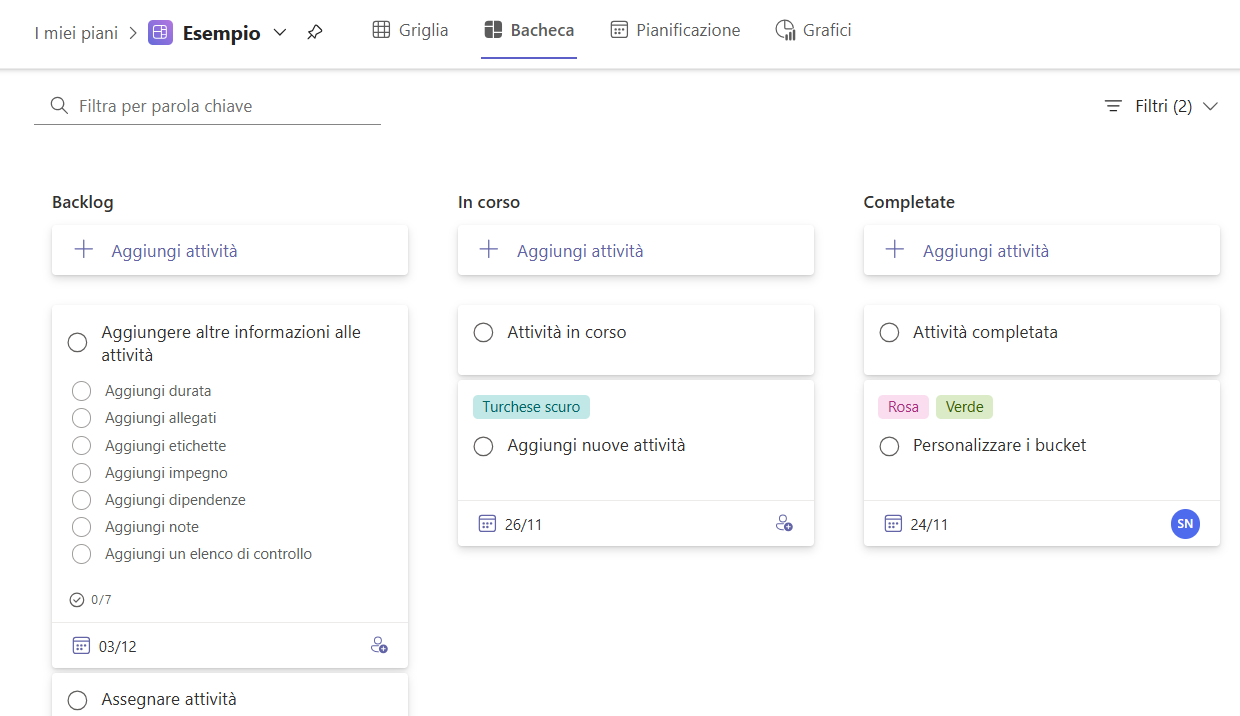
\includegraphics[width=1\columnwidth]{planner}
        \caption{Esempio di un piano di Planner} 
        \label{fig:planner}
    \end{figure}
    \item La collaborazione tra i membri del personale è agevolata da strumenti come Microsoft Teams e Outlook, i quali permettono di: scambiare ed organizzare messaggi ed \emph{e-mail}, gestire eventi come riunioni e \emph{meeting} in un apposito calendario sincronizzato ed effettuare videochiamate per agevolare l'interazione e la collaborazione tra colleghi. 
    \item Gli sviluppatori possono scegliere liberamente gli ambienti di sviluppo più adatti alle loro esigenze, anche se i principali strumenti utilizzati sono Visual Studio Code e IntelliJ IDEA, che offrono supporto per molteplici linguaggi di programmazione e \emph{framework}. 
    \item I sistemi operativi prevalentemente utilizzati in azienda sono Windows 11 e Windows 10 in modo da garantire un ambiente compatibile con la maggior parte degli strumenti \emph{software}. 
    \item Il versionamento del codice sorgente è gestito tramite Git, con il supporto di piattaforme come GitHub e GitLab, che assicurano un controllo efficace delle versioni e agevolano la collaborazione. 
    \item Per il controllo e l'automazione del ciclo di vita del \emph{software} viene utilizzato Jenkins, uno strumento che permette di ottimizzare i processi di sviluppo e distribuzione tramite \gls{Continuous Integration} e \gls{Continuous Deployment}, ovvero le pratiche di sviluppo che permettono in modo automatico, rispettivamente, una frequente integrazione del lavoro svolto e la distribuzione in ambiente di produzione dei risultati ottenuti. 
    \item La qualità del \emph{software} è garantita attraverso strumenti come SonarQube per l'analisi statica del codice, JUnit per i \emph{test} di unità ed integrazione, JMeter per i \emph{test} di carico e \emph{stress test}.\\
    Per migliorare il processo di \emph{test} viene utilizzato, dove necessario, il \emph{framework} Mockito per simulare il comportamento di specifici componenti o dipendenze esterne.\\
    Viene inoltre utilizzato lo strumento OWASP ZAP per testare il soddisfacimento di molteplici requisiti di sicurezza. 
    \item Le tecnologie principali utilizzate per la creazione e gestione della documentazione aziendale comprendono l'insieme Microsoft Office 365 mentre, per lo sviluppo \emph{software}, vengono utilizzati soprattutto il linguaggio Java e il \emph{framework} Angular. 
    \item Per la gestione e configurazione di un \emph{server web} e di basi di dati, vengono utilizzate rispettivamente Apache Web server e SQL server. 
\end{itemize}

\section{Innovazione aziendale}
L'azienda non sottovaluta l'importanza dell'innovazione in un ambiente lavorativo in costante aggiornamento come quello \gls{IT}. Lo dimostra l'importanza che viene data all'\gls{unità operativa} Ricerca e Sviluppo, alla quale ho partecipato approfondendo tecnologie nuove per l'azienda e valutando nuovi approcci organizzativi. Questi ultimi includono l'implementazione, per le nuove tecnologie adottate, di metodologie \gls{DevOps}. Tali processi atti all'automazione vengono già applicati per tecnologie consolidate aumentando l'efficacia, l'efficienza e la qualità dei lavori.\\
Wintech riconosce il valore aggiunto che i giovani possono portare e, da diversi anni, offre la possibilità di svolgere \emph{stage} universitari per formare e inserire nel mondo del lavoro studenti prossimi alla laurea.\\
Spesso, per questi ultimi, si concretizza l'opportunità di proseguire lavorativamente i rapporti con l'azienda, pertanto, il \emph{team} di sviluppo è caratterizzato da un'età media relativamente giovane, pur mantenendo al suo interno figure con consolidata esperienza.\\ 
Inoltre, al fine di accrescere le potenzialità delle proprie risorse, l'azienda fornisce corsi di formazione mirati per il personale.
